\documentclass{article}
\usepackage[utf8]{inputenc}
\usepackage{enumitem}
\usepackage{amsmath}
\usepackage{mathtools}
\usepackage{amsfonts}
\DeclarePairedDelimiter\ceil{\lceil}{\rceil}
\DeclarePairedDelimiter\floor{\lfloor}{\rfloor}
\newcommand*\xor{\mathbin{\oplus}}
\usepackage[table,xcdraw]{xcolor}
\usepackage{graphicx}
\usepackage{float}
\usepackage{amssymb}
\usepackage{adjustbox}
\usepackage{caption}
\usepackage{subcaption}
\usepackage[a4paper,margin=1in,footskip=0.25in]{geometry}
\newcommand{\xmod}[1]{\left(\bmod\ #1\right)}
\newcommand{\ximplies}{\Rightarrow\,}
\newcommand{\ncproblem}[1]{\subsection*{Problem #1}}
\newcommand{\problem}[1]{\clearpage\subsection*{Problem #1}}
\newcommand{\xbf}[1]{\mathbf{#1}}
\newcommand{\xbb}[1]{\mathbb{#1}}
\newcommand{\oa}[1]{\overrightarrow{#1}}
\newcommand{\pd}[1]{\frac{\partial}{\partial #1}}

\title{\huge{Generative Adversarial Urban Growth Prediction}}
\author{Ziad Khattab}
\date{}

\begin{document}

\maketitle

\section{Network model}

Prediction of urban growth from a sequence of satellite images requires not only the identification of growth patterns, but the ability to generate images of future maps with decently realistic quality and good enough definition to visually identify urban and non-urban areas. For this, a generative adversarial network (GAN) is used.

In a GAN, a generator network receives the history frames and attempts to provide a realistic continuation to the clip, and a discriminator network attempts to determine whether the clips it receives are real or fake, assigning a probability to the image between 0 and 1 of how likely it is to be real. The two networks compete against one another, with the generator attempting to fool the discriminator into thinking that the generated output images are areal, while the discriminator attempts to pick apart real and fake images more accurately.

\begin{figure}[H]
    \caption{graph of the generative adversarial model}
    \centering
    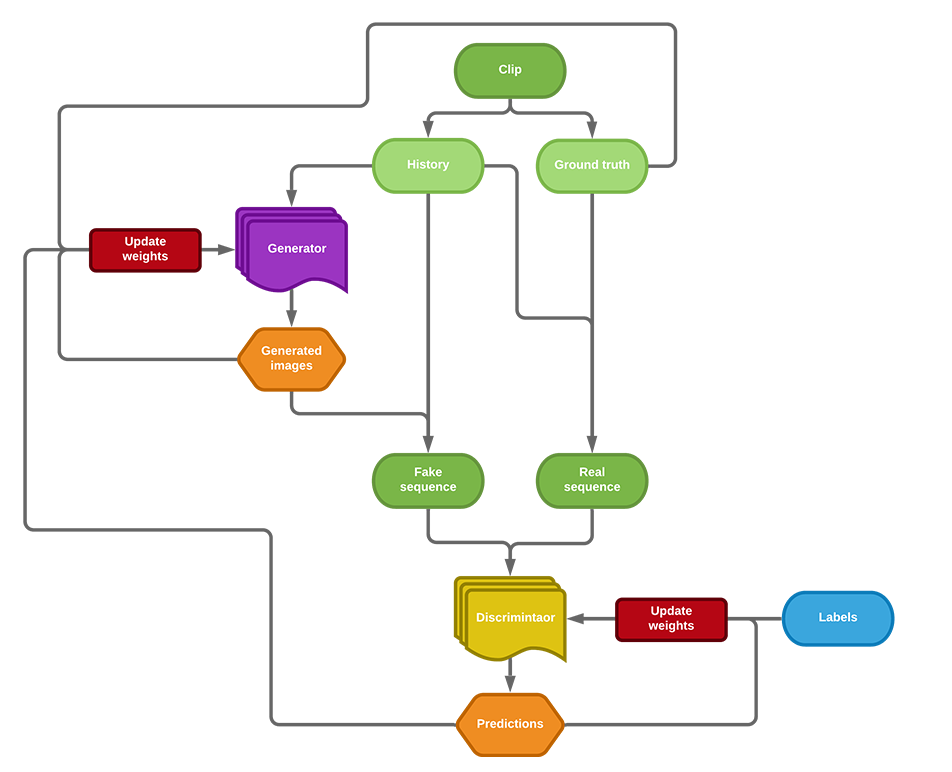
\includegraphics[width=0.7\linewidth]{gan-graph.png}
\end{figure}

\clearpage

The discriminator is a convolutional neural network image classifier that runs the clips through convolutional layers activated with ReLU, and then to fully connected layers to obtain a scalar prediction between 0 and 1. It operates on a multi-scale model, meaning that a 48 by 48 pixel square clip is downscaled to 6 by 6, 12 by 12, 24 by 24, and the original clip, and a prediction generated for each scale.

The generator is a fully convolutional image generator model that also operates with the same four-scale model. However, a significant difference from the discriminator is that the generator concatenates the upsampled output of each scale to the next one to strengthen the time dependency.

\begin{figure}[H]
    \caption{graph of the discriminator and generator models}
    \centering
    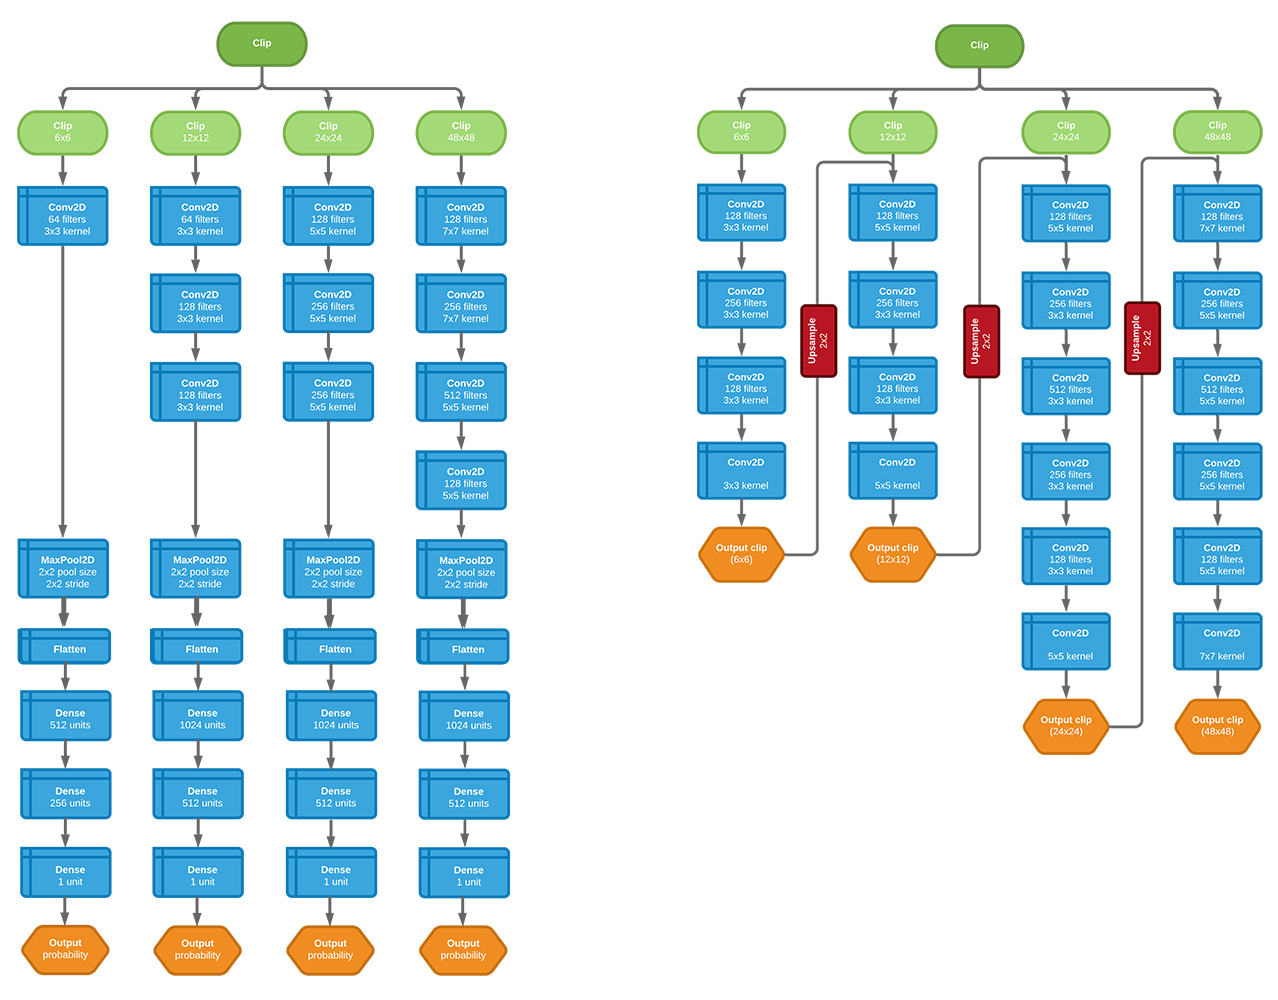
\includegraphics[width=1.0\linewidth]{disc-gen-graph.png}
\end{figure}

\clearpage

\section{Loss functions}

To mathematically define the loss functions used in training, we must first define the generator and discriminator models as functions,

\begin{align*}
    \mathrm{gen} &: \textrm{ images } \to \textrm{ images }\\
    \mathrm{disc} &: \textrm{ images } \to [0, 1]
\end{align*}

\subsection{$\ell_p$ loss}

We define the $\ell_p$ loss as,

\begin{align*}
    \ell_p(x, y) = |x - y|^p,\; p \in \big\{1, 2\big\}
\end{align*}

This loss represents either the absolute difference (if $p = 1$), or the absolute squared difference (if $p = 2$) between the generated images $x$ and the ground truth images $y$. This is the simplest metric for the accuracy of the generated images.

\subsection{Adversarial loss}

First, define the binary crossentropy loss as,

\begin{align*}
    \mathrm{bce}(y, y') = -\sum_i y_i\log(y_i') + (1-y_i)
    \log(1-y_i')
\end{align*}

where $y$ represents the predicted labels given as output of the discriminator, and $y'$ represents the true labels assigned to the data. For each generate image that the discriminator receives, it generates a probability that this image matches the ground truth image. The binary crossentropy loss is a measure of how close this probability is to the truth. It operates on a logarithmic basis, so probabilities that are the same as the true label have a very small loss, while probabilities that are very far from the true label have an enormous loss.

Next, we define the discriminator loss,

\begin{align*}
    \mathrm{loss}_{\mathrm{disc}}(x, y) =
    \mathrm{bce}(\mathrm{disc}(x, y), 1) +
    \mathrm{bce}(\mathrm{disc}(x, \mathrm{gen}(x)), 0)
\end{align*}

\subsection{Discriminator loss}

The loss used for the discriminator is defined as,

\begin{align*}
    \mathrm{adv}(x, y) =
    \mathrm{bce}(\mathrm{disc}(x, \mathrm{gen}(x)), 0)
\end{align*}

\subsection{Gradient difference loss (GDL)}

Define the image GDL as,

\begin{align*}
    \mathrm{gdl}(x, y) = \sum_{i, j}\left||y_{i, j} - y_{i - 1, j}| -
    |\mathrm{gen}(x)_{i, j} - \mathrm{gen}(x)_{i - 1, j}|\right|^c\\
    + \left||y_{i, j - 1} - y_{i, j}| -
    |\mathrm{gen}(x)_{i, j - 1} - \mathrm{gen}(x)_{i, j}|\right|^c
\end{align*}

This is used to penalize images that are significantly blurry and fuzzy, to improve definition of the final predicted image. The value of $c$ is a constant to be determined through arbitrary choice or fine tuning. For the purposes of the \texttt{dohamaps} model, the value of $c = 1$ was used.

\subsection{Generator loss (combined)}

Finally, the combined loss, which is used as the loss for the generator,

\begin{align*}
    \mathrm{loss}_{\mathrm{gen}}(x, y) = \alpha\, \mathrm{adv}(x, y) +
    \beta\, \mathrm{\ell}_p(x, y) + \gamma\, \mathrm{gdl}(x, y)
\end{align*}

Once again, the values of $\alpha,$ $\beta,$ and $\gamma$ are constants, which in the \texttt{dohamaps} model were set to $\alpha = 0.05,$ $\beta = 1,$ and $\gamma = 1$.

\section{Metrics}

In addition to the loss functions, the model contains metrics. These metrics do not directly inform the training loop, but are reported regularly to provide measures of the model's performance.

\subsection{Peak signal to noise ratio (PSNR)}

The PSNR is defined as,

\begin{align*}
    \mathrm{psnr}(x, y) = 10 \cdot \log_{10}\left( \frac{N \cdot
    \mathrm{max}}{\sum (x_i - y_i)} \right)
\end{align*}

where $N$ is the number of channels, and $\mathrm{max}$ is the maximum value of the image signal. In a default RGB image, this value is 255. The PSNR is measured in decibels, where a higher value indicates an image that is harder to distinguish from the original by the naked eye.

\subsection{Sharpness difference}

The sharpness difference is defined as,

\begin{align*}
    \mathrm{sharpdiff}(x, y) = 10 \cdot \log_{10}\left(\frac{N \cdot
    \mathrm{max}^2}{\sum_i \sum_j |(\Delta_i x + \Delta_j x) - (\Delta_i
    y + \Delta_j y)|}\right)
\end{align*}

which measures the loss of sharpness between the true frame $x$ and the predicted image $y$.

\subsection{Structural similarity index measure (SSIM)}

Define the SSIM (Wang et. al) as,

\begin{align*}
    \mathrm{ssim}(x, y) = \frac{(2\mu_x\mu_y + c_1)(2\sigma_{xy} + c_2)}
    {(\mu_x^2 + \mu_y^2 + c_1)(\sigma_x^2 + \sigma_y^2 + c_2)}
\end{align*}

where $\mu_x$ is the average of image $x$, and $\mu_y$ is the average of image $y$, $\sigma_x$ and $\sigma_y$ are the variance of $x$ and $y$, $\sigma_{xy}$ is the covariance of $x$ and $y$, and $c_1$ and $c_2$ are constants.

\section{Hyperparameters}

In addition to the losses and metrics defined above, there are several significant hyperparameters that can heavily influence the training and outputs of the model. The generator and the discriminator both use the Adam optimizer (Kingma et. al), which has takes as its main parameter the learning rate. Learning rates that are too high will cause the loss to oscillate and lead to inaccurate results, while learning rates that are too low will not converge in a reasonable amount of time.

The next pair of hyperparameters are the history and prediction length. The history length represents the length of the clip taken as an input to the generator, while the prediction length represents the length of the clip output as a prediction. Predictions beyond the length of the prediction clip are computed recursively from initial prediction. Image sequences that change over time, but not necessarily in a strongly time-linked pattern, benefit from a shorter history and prediction length. For the purposes of urban growth, where time-linked patterns are important, longer history and prediction lengths are beneficial.

The final hyperparameter is the size of the clips that the input images are cropped to due to memory constraints. Clips that are smaller in size will allow the model to capture more detailed features and output images with higher definition, but will miss out on larger image features that are obtained from larger clips.

The following table displays the values of all these hyperparameters in the \texttt{dohamaps} model.

\begin{table}[h]
\begin{tabular}{ll}
\textbf{Hyperparameter} & \textbf{Value}\\
Generator learning rate & 0.0000085\\
Discriminator learning rate & 0.000005\\
History length & 8 frames\\
Prediction length & 16 frames\\
Clip size & 64 $\times$ 64\\
\end{tabular}
\end{table}

\end{document}
